\documentclass[tikz,border=8pt]{standalone}
\usetikzlibrary{calc}
\begin{document}
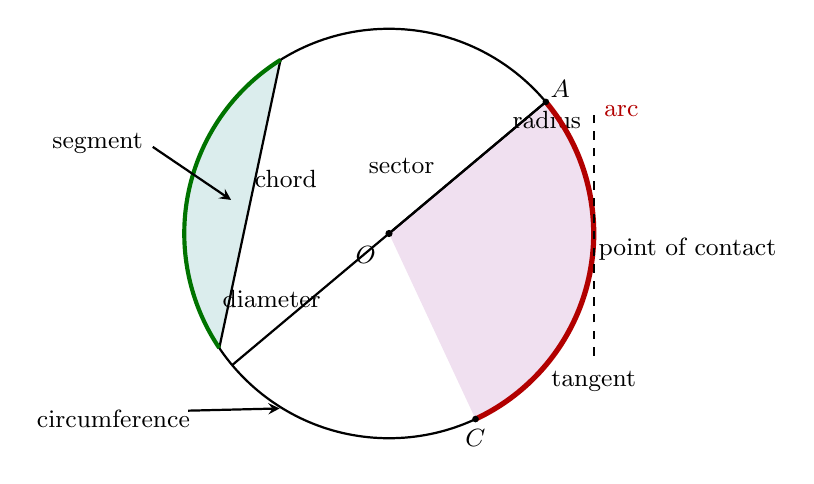
\begin{tikzpicture}[font=\small,>=stealth,line width=0.8pt]
  \coordinate (O) at (0,0);
  \fill[violet!12] (O) -- (40:2.6) arc[start angle=40, end angle=-65, radius=2.6] -- cycle;
  \fill[teal!14] (122:2.6) arc[start angle=122, end angle=214, radius=2.6] -- cycle;
  \draw (O) circle (2.6);
  \coordinate (A) at (40:2.6);
  \coordinate (A2) at (220:2.6);
  \coordinate (C) at (-65:2.6);
  \coordinate (D) at (0:2.6);
  \coordinate (J) at (122:2.6);
  \coordinate (K) at (214:2.6);
  \draw (O) -- (A) node[pos=0.74, above right=-1pt] {radius};
  \draw (A) -- (A2) node[pos=0.72, below left=-4pt] {diameter};
  \draw (J) -- (K) node[pos=0.45, above right=-3pt] {chord};
  \draw[green!45!black, line width=1.5pt] (J) arc[start angle=122, end angle=214, radius=2.6];
  \draw[red!70!black, line width=1.9pt] (40:2.6) arc[start angle=40, end angle=-65, radius=2.6];
  \node[red!70!black] at (2.95,1.55) {arc};
  \node at (-3.7,1.15) {segment};
  \draw[->] (-3.0,1.1) -- (168:2.05);
  \node at (0.16,0.86) {sector};
  \draw[dashed] (2.6,-1.55) -- (2.6,1.55);
  \node[below] at (2.6,-1.62) {tangent};
  \node[below right=-2pt] at (D) {point of contact};
  \node[below left=1pt] at (O) {$O$};
  \fill (O) circle (1.3pt);
  \fill (A) circle (1.2pt) node[above right=-2pt] {$A$};
  \fill (C) circle (1.2pt) node[below] {$C$};
  \node at (-3.5,-2.35) {circumference};
  \draw[->] (-2.55,-2.25) -- (-122:2.62);
\end{tikzpicture}
\end{document}
